
\documentclass[letterpaper, 10 pt, conference]{ieeeconf}  % Comment this line out if you need a4paper
\usepackage{graphicx}



%\documentclass[a4paper, 10pt, conference]{ieeeconf}      % Use this line for a4 paper

\IEEEoverridecommandlockouts                              % This command is only needed if 
                                                          % you want to use the \thanks command

%\overrideIEEEmargins                                      % Needed to meet printer requirements.

% See the \addtolength command later in the file to balance the column lengths
% on the last page of the document

% The following packages can be found on http:\\www.ctan.org
%\usepackage{graphics} % for pdf, bitmapped graphics files
%\usepackage{epsfig} % for postscript graphics files
%\usepackage{mathptmx} % assumes new font selection scheme installed
%\usepackage{times} % assumes new font selection scheme installed
%\usepackage{amsmath} % assumes amsmath package installed
%\usepackage{amssymb}  % assumes amsmath package installed
\usepackage{cite}
\usepackage{mathtools}
\usepackage{cleveref}
\usepackage{amsmath}
\graphicspath{{./pictures/}}
%\addtolength{\belowcaptionskip}{-100pt}
\addtolength{\abovecaptionskip}{-10pt}

\title{\LARGE \bf
Magnetic Hammer Actuation for Tissue Penetration using a Millirobot}


\author{Julien Leclerc, Ashwin Ramakrishnan, Nikolaos V. Tsekos, and Aaron T. Becker % <-this % stops a space
\thanks{This work was supported by the National Science Foundation, Grant No. 1646566. }% <-this % stops a space
\thanks{Authors are with the Dept. of Electrical and Computer
Engineering, University of Houston, Houston, TX 70004, USA
        {\tt\small jleclerc@uh.edu}}%
\thanks{The authors would like to thank Ouajdi Felfoul for designing and running the MRI pulse sequences. They are also grateful to Jarrett Lonsford and Javier Garcia who performed the coefficient of restitution measurements.}
%\thanks{$^{2}$Bernard D. Researcheris with the Department of Electrical Engineering, Wright State University,
%       Dayton, OH 45435, USA
%      {\tt\small b.d.researcher@ieee.org}}%
}


\begin{document}



\maketitle
\thispagestyle{empty}
\pagestyle{empty}


%%%%%%%%%%%%%%%%%%%%%%%%%%%%%%%%%%%%%%%%%%%%%%%%%%%%%%%%%%%%%%%%%%%%%%%%%%%%%%%%
\begin{abstract}

Untethered magnetic navigation of millirobots within a human body using a Magnetic Resonance Imaging (MRI) scanner is a promising technology for minimally invasive surgery or drug delivery.
Because MRI scanners have a large static magnetic field, they cannot generate torque on magnetic millirobots and must instead use gradient-based pulling.
 However, gradient values are too small to produce forces large enough to penetrate tissue. 
 This paper presents a method to produce large pulsed forces on millirobots. 
 A ferromagnetic sphere is placed inside a hollow robot body and can move back and forth. 
 This movement is created by alternating the magnetic gradient direction. 
 On the posterior side, a spring allows the sphere to change direction smoothly. 
 On the anterior side, a hard rod creates a surface for the sphere to impact. 
 This impact results in a large pulsed force. 
 The purpose of this study was to understand the functioning of magnetic hammer actuation and control, as well as demonstrate the viability of this mechanism for tissue penetration.
 This paper begins with modeling and simulating this system. 
 Next, different control strategies are presented and tested. The system successfully penetrated lamb brain samples.
  Finally, preliminary tests inside a clinical MRI scanner demonstrate the potential of this actuation system. 

\end{abstract}


%%%%%%%%%%%%%%%%%%%%%%%%%%%%%%%%%%%%%%%%%%%%%%%%%%%%%%%%%%%%%%%%%%%%%%%%%%%%%%%%
\section{INTRODUCTION}

The navigation of millimeter-scale robots through the passageways of bodies is currently being studied as a method to perform highly localized drug delivery or perform minimally invasive surgery \cite{7067029,702,mi2020295}. Untethered navigation can be achieved by placing a ferromagnetic piece inside the robot and producing a controlled magnetic field around a patient. Propulsion and steering of millirobots can be accomplished by either moving a permanent magnet assembly around a patient \cite{taylor} or by controlling the current inside electromagnets \cite{MRM21638}. The latest solution is often realized with an MRI scanner which already includes several electromagnets. In an MRI, the background field magnetizes the ferrous components of the robot, and the gradient coils generate the magnetic gradient necessary to produce forces. 
The Magnetic Resonance Imaging (MRI) scanner can be used simultaneously to provide real-time imaging of the operating area as well as positioning of the robot.\par
The force generated on the millirobots is proportional to the gradient field  strength. 
Commercial MRI scanners produce gradients in the range of 20 to 40 mT/m. 
These gradients are sufficient to maneuver milli-robots inside fluid-filled regions of the body, such as vessels, \cite{martel2007automatic} but insufficient for tissue penetration that requires larger forces \cite{7139341}; tissue penetration is required for many procedures, including brachytherapy and micro-biopsy.
The purpose of this paper is to present and study a method, denoted  \emph{magnetic hammer actuation}, that can generate large pulsed forces for tissue penetration. The paper demonstrates the capability of the device to penetrate tissue and shows that an MRI scanner is suitable to produce the external magnetic field and gradient necessary for the actuation.
The magnetic hammer is a system embedded into the millirobot. 
The millirobot has a tubular structure in which a ferromagnetic sphere can move back and forth.
 This movement is produced by alternately changing the gradient direction. 
 On the posterior side of the millirobot, a spring allows the sphere to change direction smoothly. 
 On the anterior side, a hard rod creates a surface for the sphere to impact, the \emph{impact plate}.
  This impact results in large pulsed forces that enable penetrating body tissues progressively.
A magnetic test bench has been developed to make experimental tests more practical and less expensive.
 It includes coils, sensors, power electronics, and a real-time controller.\par
The paper studies three control strategies. The open-loop control switches the magnetic gradient direction at constant frequency. It is completely independent of the sphere position and uses no feedback. The partially closed-loop control detects the impact of the sphere and switches the magnetic gradient direction as soon as the impact is detected. The original gradient direction is reapplied after a constant time $t_s$. The perfect closed-loop control assumes a theoretical sensor able to measure the position of the sphere at any time. It is capable of detecting the impact of the sphere as well as the change of direction on the posterior side. The controller is therefore able to change the direction of the gradient when the impact is detected and when the change of direction on the posterior side is detected.\par


\begin{figure}\centering
  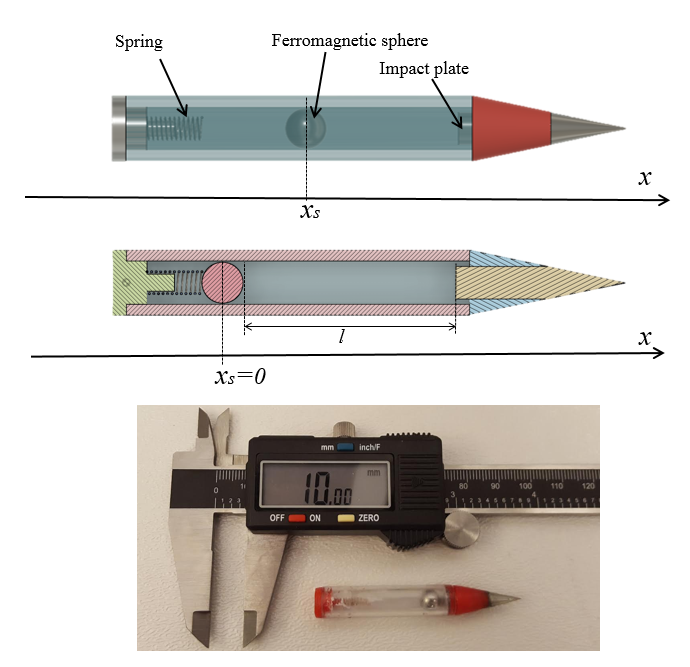
\includegraphics[width=220pt]{figure1-2.png}
  \caption{Schematic representation of a millirobot actuated by a magnetic hammer.}
  \label{millirobot}
  %\vspace{-2em}
\end{figure}

\begin{figure}
\begin{centering}
  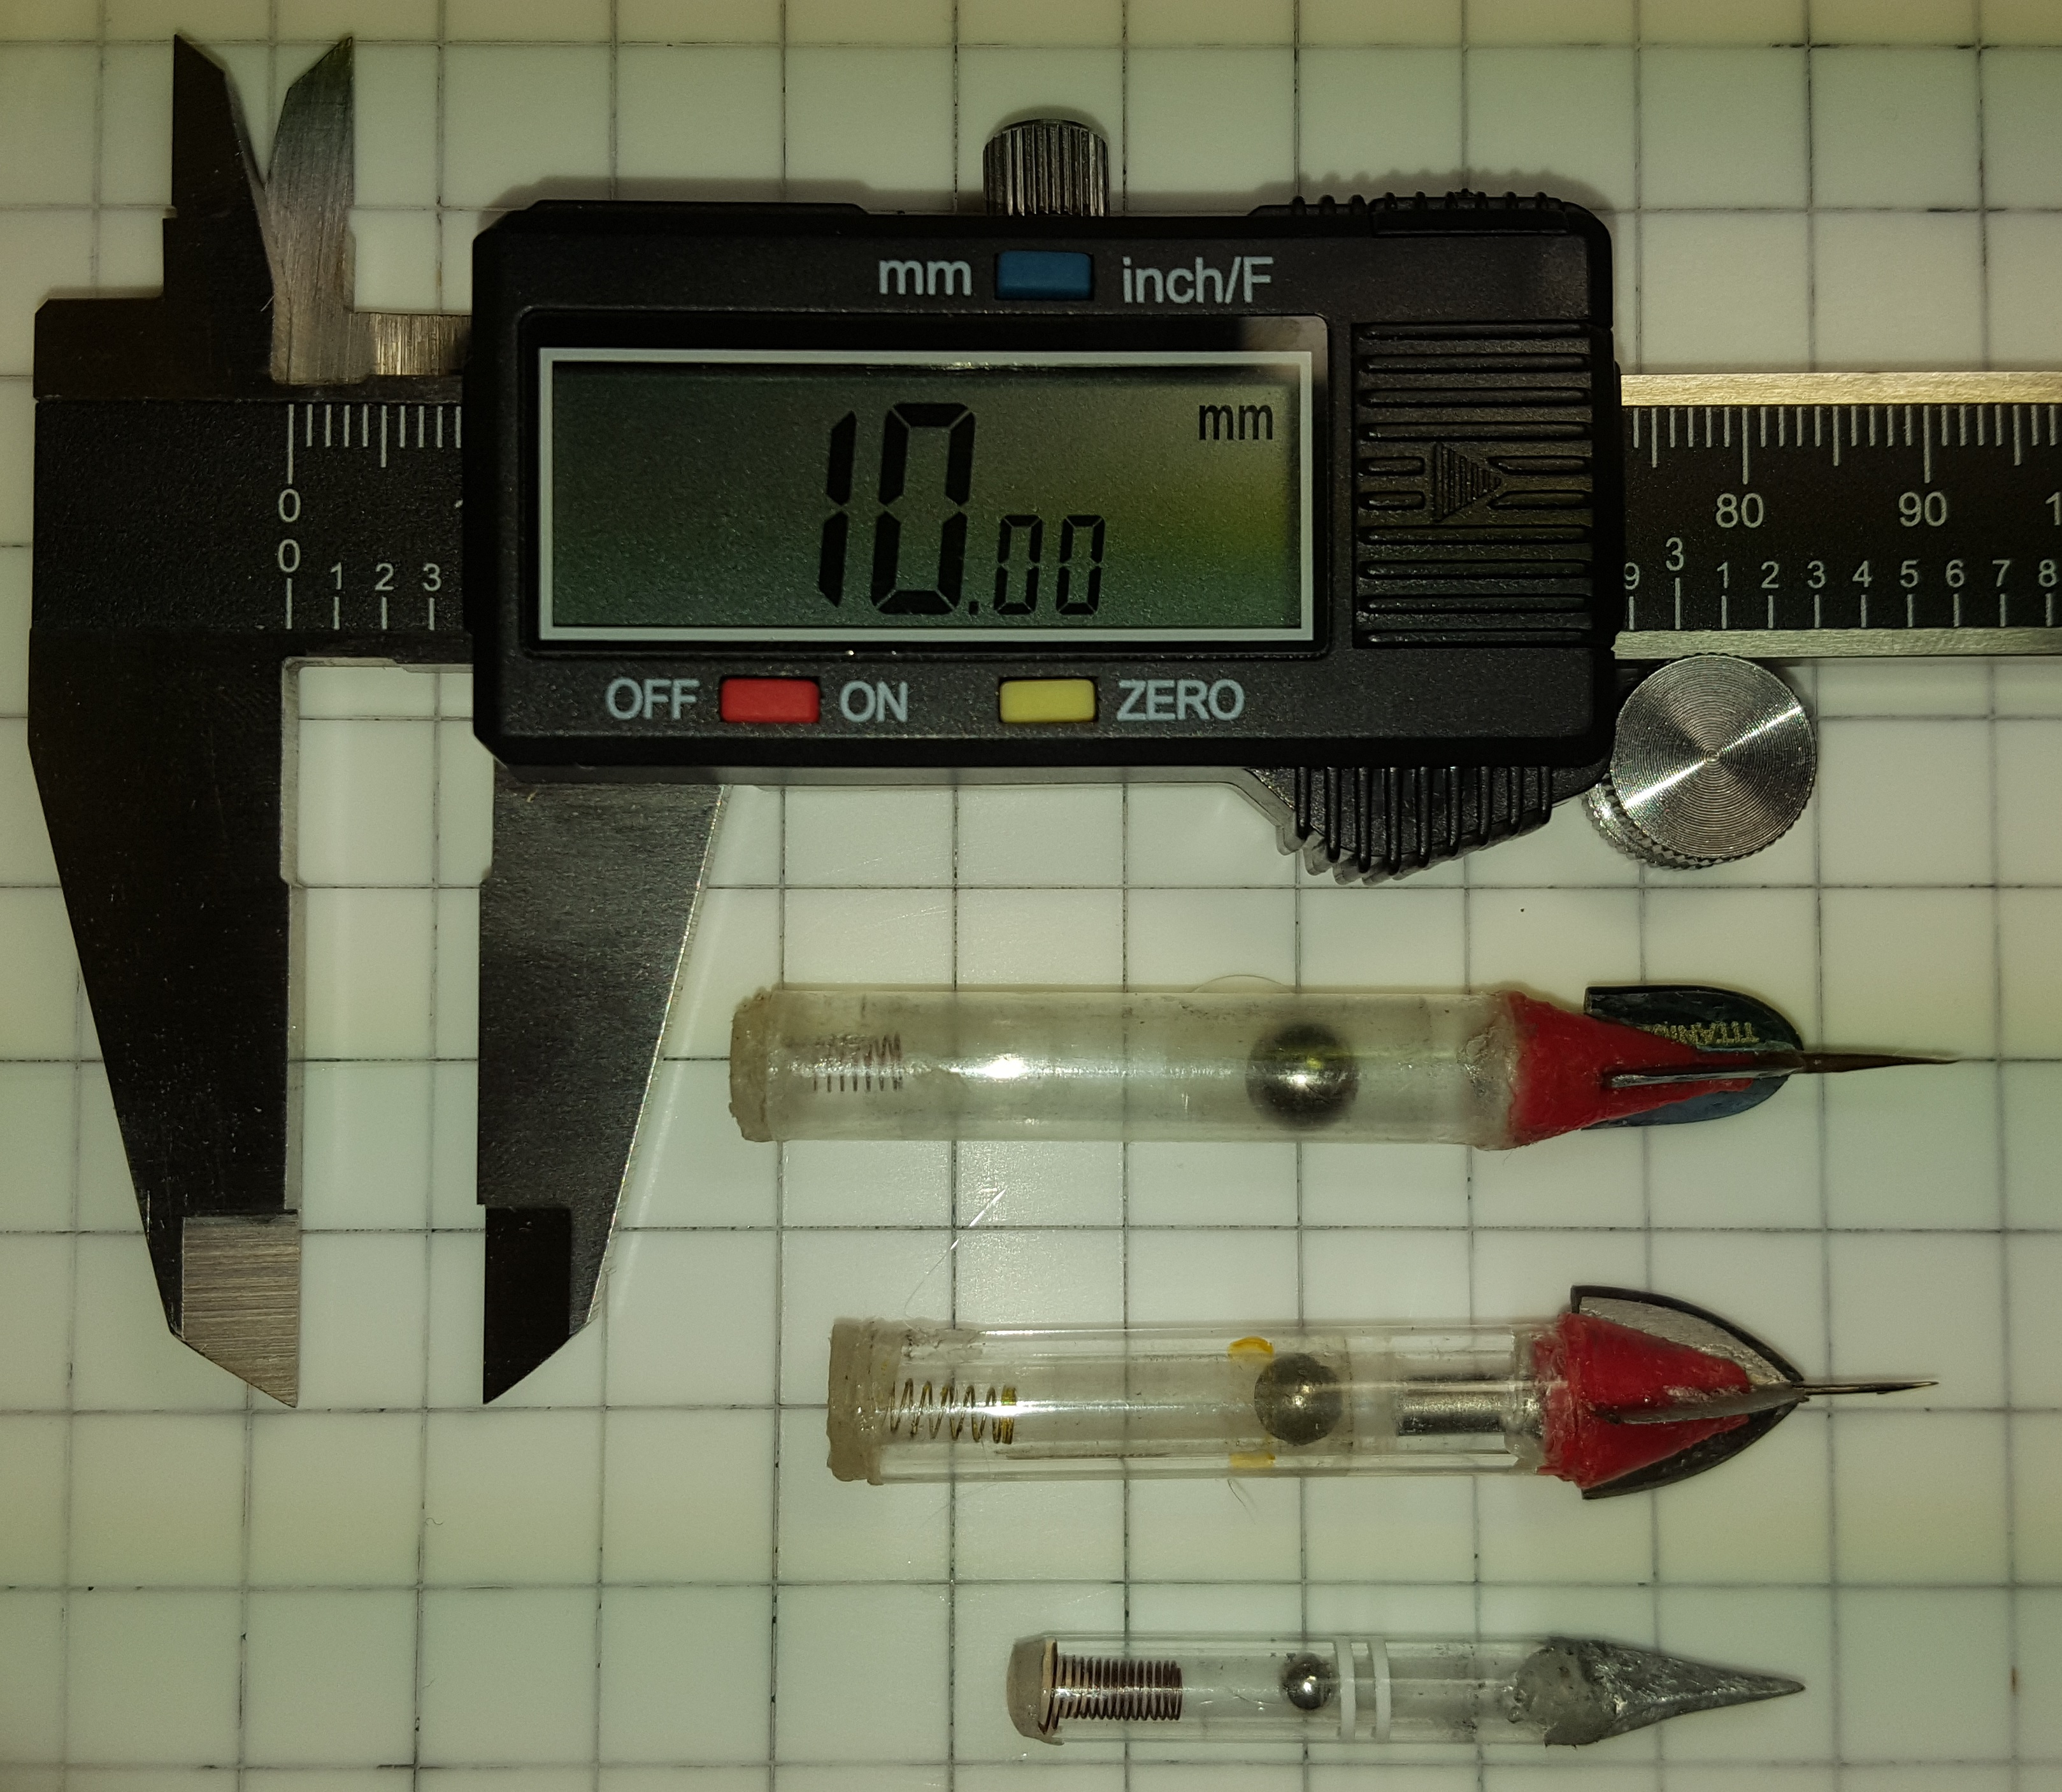
\includegraphics[width=120pt]{robots_prototypes.jpg}
  \caption{Picture of three millirobot prototypes actuated by a magnetic hammer.}
  \label{prototypes}
  %\vspace{-2em}
\end{centering}
\end{figure}

The paper is organized as follows: first, the system is mathematically modeled, and its behavior is studied in Section \ref{theoretical}. Secondly, parameters for the model are experimentally measured (see Section \ref{cor_det}). Different materials for the impact plate are compared. Thirdly, the magnetic test bench is described and the test of a magnetic hammer is presented (see \cref{experiment}). Next, preliminary results from an open-loop test performed in a clinical MRI scanner are presented in Section \ref{MRI_tests}. The last Section (Section \ref{conclusion}) is a conclusion of this study.


\section{Theoretical study}
\label{theoretical}
\subsection{Mechanical modelization}
The motion of the sphere between two consecutive impacts can be divided into two  phases, based on the forces that act on it. The magnetic gradient force $F_{\textrm{mag}}$ and friction force $F_{\textrm{friction}}$ act on the sphere during its motion along the free length of the tube, $L$ (see Fig. \ref{FBD} (i),(iii)). When the spring is compressed, its reaction force $F_{\textrm{spring}}$ acts on the ball as well (see Fig. \ref{FBD} (ii)). The directions of $F_{\textrm{mag}}$ and $F_{\textrm{friction}}$  change depending on the direction of motion of the sphere. 
\begin{figure}
	\begin{centering}
	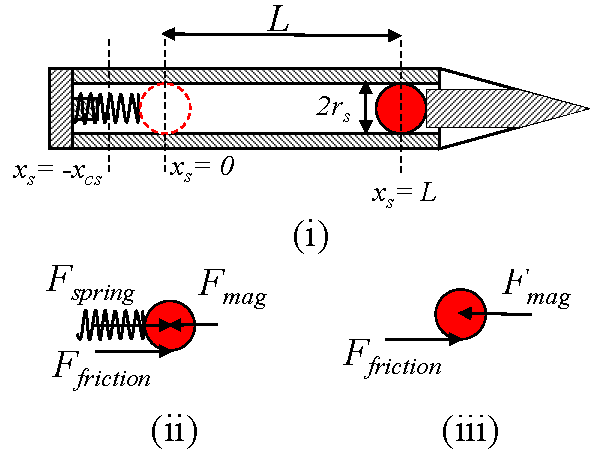
\includegraphics[width=150pt]{FBD_R1.pdf}
	\caption{(i) Free length of sphere travel, $L$; (ii) free body diagram of sphere when spring is compressed, (iii) when spring is not compressed.}
	\label{FBD}
	\end{centering}
%	\vspace{-2em}
	\end{figure}
Inside the homogeneous region of an MRI scanner, the magnitude of $F_{\textrm{mag}}$ is constant \cite{CMR:CMR20163}. The same has been assumed for developing analytical and numerical models in this paper. The formula for calculating $F_{\textrm{mag}}$ is presented in Section II-B. Friction is considered negligible, but this assumption will be relaxed in later sections. The spring force is given by
\begin{equation}
F_{\text{spring}}=k x,
\label{spring_force}
\end{equation}
where $x$ is the compression length, and $k$ is the spring constant. In the case of perfect closed-loop control, the magnetic gradient direction is changed when the sphere hits the impact plate and when the sphere velocity slows to zero when it compresses the spring. These two events represent the instances when the sphere changes direction. In other words, to maximize the impact velocity, the magnetic force, and therefore, the magnetic gradient, are oriented in the same direction as the sphere velocity vector. In the simulations, the sphere changes direction after impact, and after the full compression of the spring. The perfect closed-loop system can therefore be easily modeled by applying a magnetic gradient that is always in the same direction as the sphere velocity.

An analytical model was developed by solving the system of differential equations describing the dynamics of sphere motion. This model allows predicting the impact velocity for each impact, given a set of input parameters. The sphere-impact plate system is assumed to have a coefficient of restitution, $e$. This model assumes that the robot capsule does not move. As seen in \cref{Closedloop_Impact_velocity}, the impact velocity initially increases and ultimately saturates for all values of $e$ greater than 0 and less than or equal to 1. The system reaches a resonant state when the impact velocity saturates. This happens when the energy lost by the sphere during impact equals the energy gained by it during the rest of the cycle. A higher $e$ results in a higher impact velocity. For $e$ = 1, the impact velocity indefinitely increases since there is no energy loss during impact. An analytical formula was derived to predict the resonant impact velocity for a given set of input parameters and for values of $e$ between 0 and 1. This was done by solving for the impact velocity at resonance, under the condition that the velocities at impacts $i$ and $i+1$ are equal. Using this condition, \cref{Resonant_CLvelocity} is derived by solving the differential equations that define the dynamics of sphere motion between impacts. The magnetic gradient is always in the same direction as the sphere velocity vector. The results given by \cref{Resonant_CLvelocity} were also verified by numerical simulations in {\sc Matlab}.
\begin{figure}
	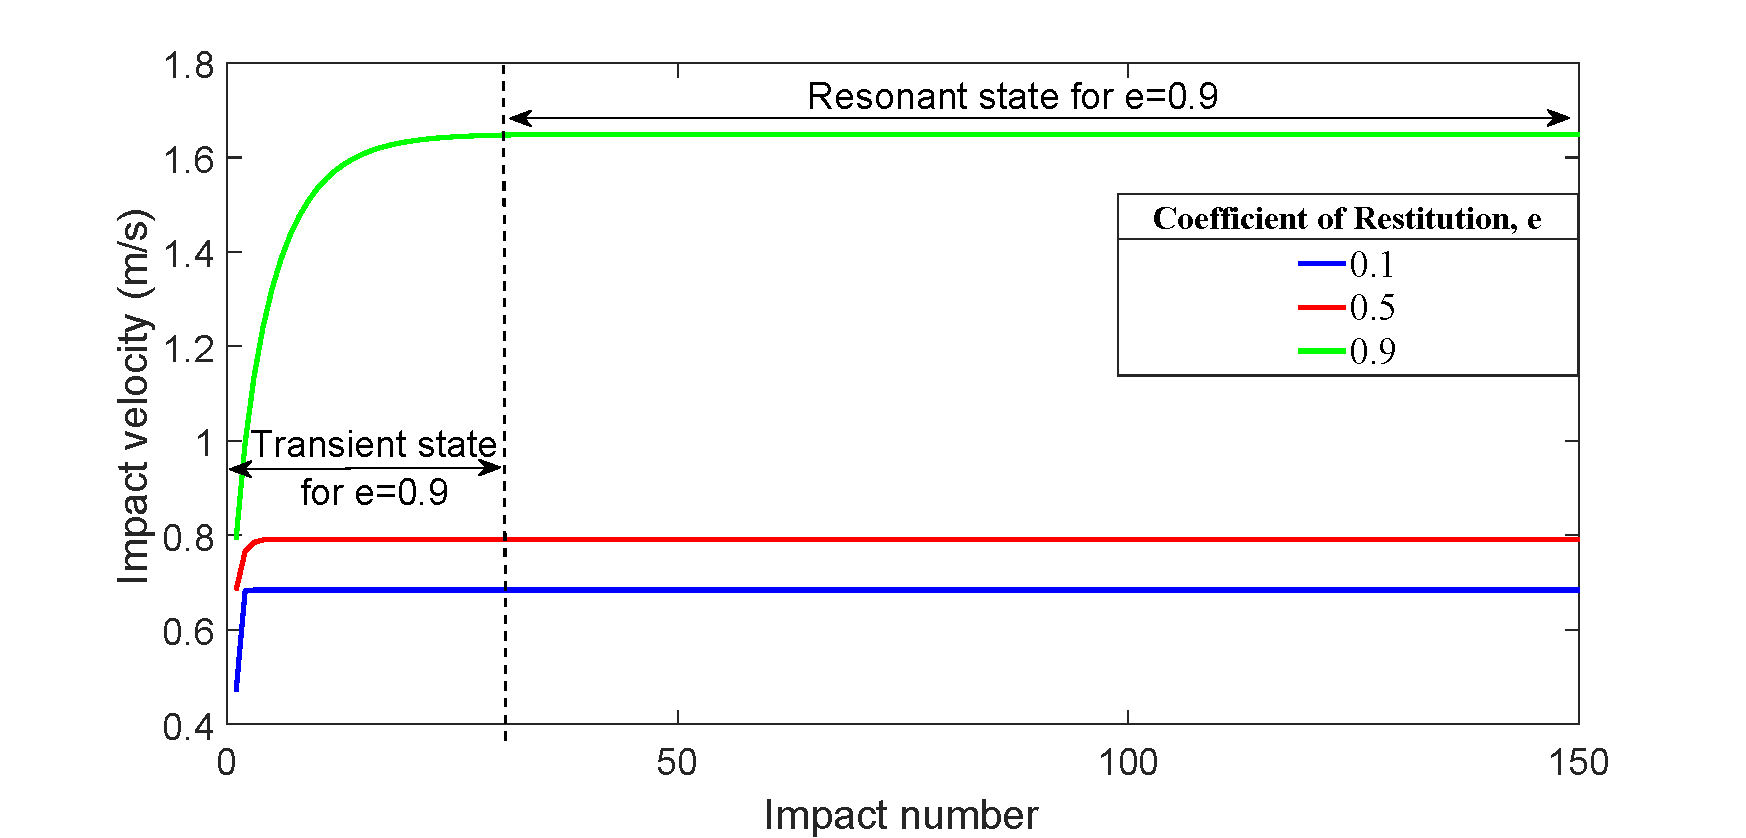
\includegraphics[width=\linewidth]{Closedloop_Impact_velocity.pdf}
	\caption{Closed-loop impact velocity for 150 impacts; $k$ = 50 N/m; $F_{\textrm{mag}}$ = 1.5e-3 N; $L$ = 0.03 m; $m_s$ = 5.58e-4 kg; $r_s$ = 2.5 mm.}
	\label{Closedloop_Impact_velocity}
	%\vspace{-1.5em}
	
\end{figure}
\begin{equation}
\resizebox{\linewidth}{!}
{$
	v_{\text{res}}=\frac{2 \sqrt{\frac{F_{\text{mag}} \left(\left(e^2+1\right) F_{\text{mag}}+\left(e^2-1\right) (-k) L+\sqrt{\left(2-2 e^4\right) k L F_{\text{mag}}+\left(1+e^2\right)^2 F_{\text{mag}}^2}\right)}{k m_s}}}{1-e^2}
	$}
\label{Resonant_CLvelocity}
\end{equation}

In the above equation, $m_s$ is the mass of the sphere in kg. The radius of the ball $r_s$ indirectly influences the impact velocity through $F_{\textrm{mag}}$ and $m_s$, both of which depend on the volume of the sphere. The variation of $v_\text{res}$ with changes in $L,e,k,m_s,r_s,F_{\textrm{mag}}$ were plotted and they were all found to be monotonic functions with no critical points. In \cref{Resonant_CLvelocity}, $v_\text{res}$ tends towards infinity as $e$ tends to 1. In this case there is no loss of energy during collision and hence, the impact velocity indefinitely increases with subsequent impacts. Further, the time between impacts at resonance, $t_\text{res}$, is a constant value and is given by \cref{tres6}. $t_\text{res}$ is calculated by adding up the time taken for the sphere to travel through each of the four phases of motion defined in the introduction to eqn. \ref{Resonant_CLvelocity}. The values $t_{\text{pos},1}$, $t_{\text{pos},2}$, $t_{\text{ant},1}$ and $t_{\text{ant},2}$ represent the time for the sphere to move from $x_s =$ (i) $L$ to 0, (ii) 0 to $-x_{cs}$, (iii) $-x_{cs}$ to 0, and (iv) 0 to $L$, all in a perfect closed-loop system with optimal gradient switching. Here, $x_{cs}$ is the maximum compression distance of the spring (See Fig. \ref{FBD} (i)). The durations of motion for each of these individual phases are calculated by solving the equations of motion with the forces acting as shown in \cref{FBD}. Friction has been assumed to be negligible for these calculations.

\begin{align}
\label{tres6}
t_\text{res}&=t_{\text{pos},1}+t_{\text{pos},2}+t_{\text{ant},1}+t_{\text{ant},2}\\
%\end{equation}
%\begin{equation}
\label{tres1}
t_{\text{pos},1}&=\frac{\sqrt{e^2 v_{\text{res}}^2+\frac{2 L F_{\text{mag}}}{m_s}}-e v_{\text{res}}}{\frac{F_{\text{mag}}}{m_s}}\\
t_{\text{pos},2}&=\frac{\pi -\tan ^{-1}\left(\frac{k \sqrt{e^2 v_{\text{res}}^2+\frac{2 L F_{\text{mag}}}{m_s}}}{\omega  F_{\text{mag}}}\right)}{\omega } ; \text{$\omega $ = }
\sqrt{\frac{k}{m_s}}
\label{tres2}\\
t_{\text{ant},1}&=\frac{\cos ^{-1}\left(\frac{F_{\text{mag}}}{F_{\text{mag}}+k x_{cs}}\right)}{\omega }
\label{tres3}\\
t_{\text{ant},2}&=\frac{v_{\text{res}}-\sqrt{v_{\text{res}}^2-\frac{2 L F_{\text{mag}}}{m_s}}}{\frac{F_{\text{mag}}}{m_s}}
\label{tres4}\\
x_{cs}&=\frac{\sqrt{e^2 k m_s v_{\text{res}}^2+2 k L F_{\text{mag}}+F_{\text{mag}}^2}+F_{\text{mag}}}{k}
\label{tres5}
\end{align}
%\end{left}
\begin{figure}\centering
	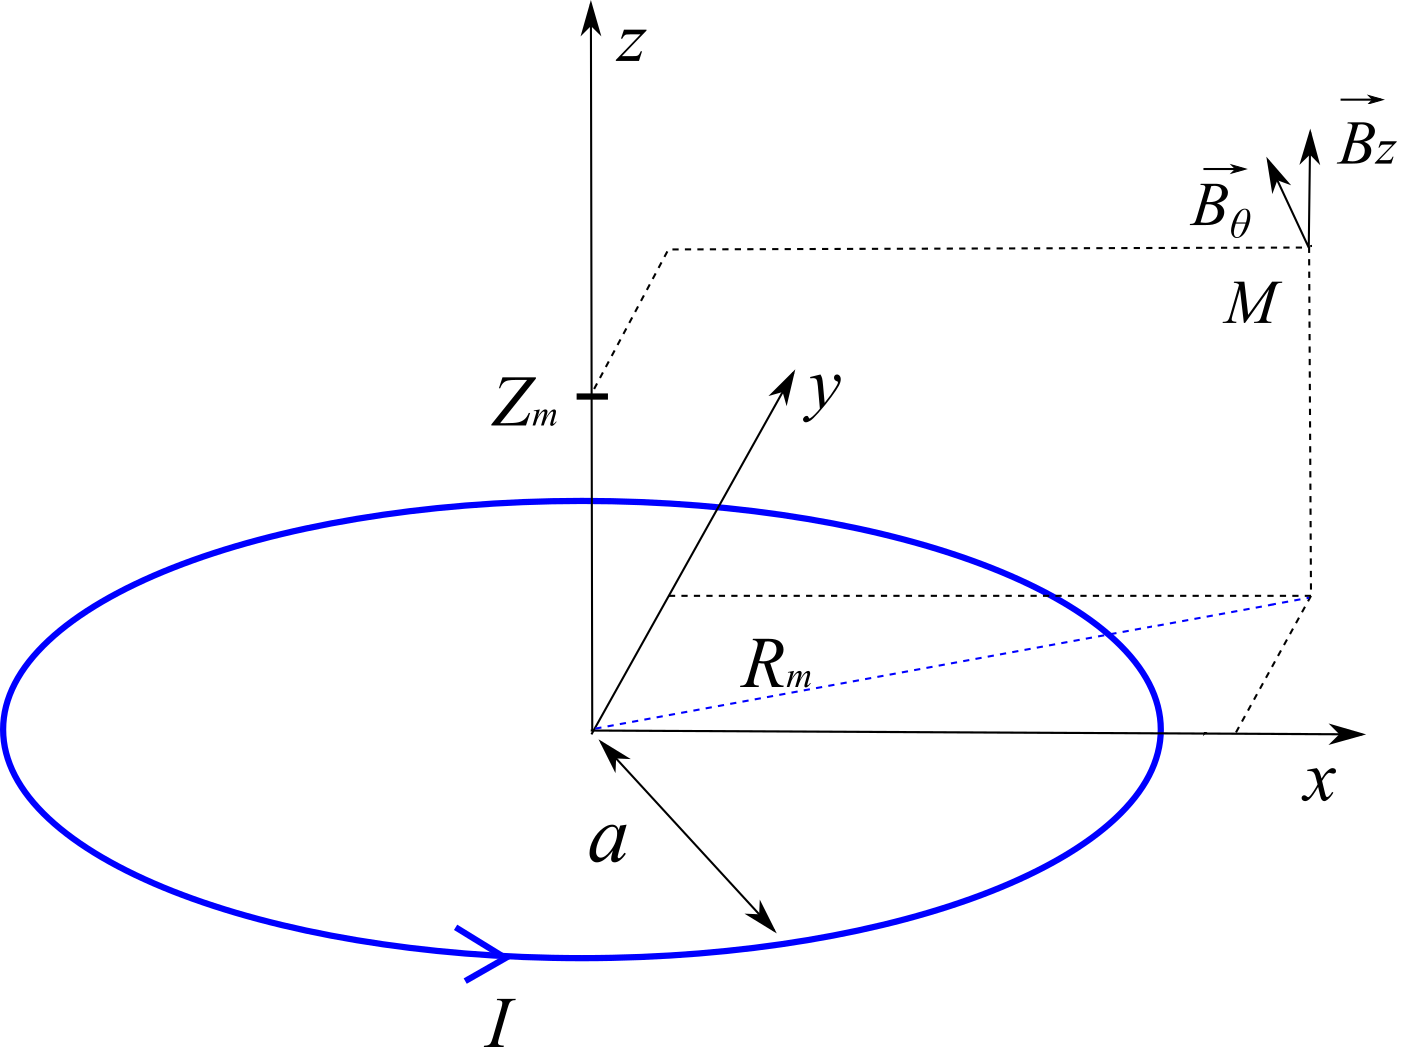
\includegraphics[width=140pt]{single_loop.png}
	\caption{Geometry and variables used in equation \cref{Bz1loop,Bteta1loop,delta,beta}}
	\label{single_loop_geometry}
	%\vspace{-1em}
\end{figure}

\begin{figure}\centering
	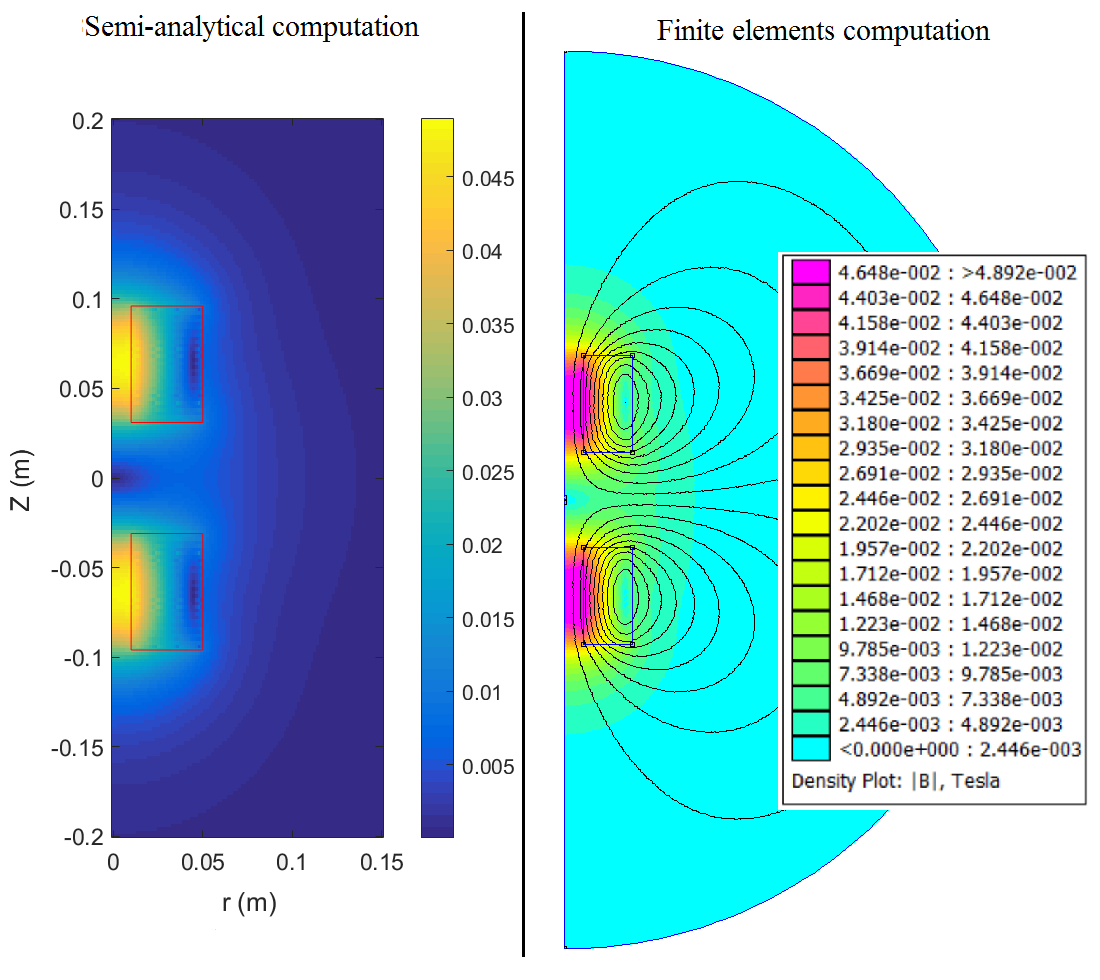
\includegraphics[width=220pt]{Femm_matlab_comparison.png}
	\caption{Comparison between the flux density computed with the semi-analytical method with {\sc Matlab} and the flux density computed via a finite element method with FEMM. The maximum difference is 0.8 \%.}
	\label{Femm_matlab_comparison}
	%\vspace{-1.9em}
\end{figure}

In the above equations, $\omega$ represents the natural frequency of the spring-mass system. The value of $x_{cs}$ can be used to select an appropriate free length for the spring, to ensure that it does not bottom out during compression. 
%\vspace{-2em}
\subsection{Magnetic field calculation}
\label{magfield}
The magnetic field generated by an MRI scanner can be separated into two components. The first is a constant and strong magnetic field $B_0$ along the z-axis. This field is used to align the magnetic moments of the protons. Commercial MRI scanners have $B_0$ typically ranging from 1.5 to 3 T. The second component of the field is the magnetic gradient. It is used to encode the MRI signal spatially. The flux density $\mathbf{G}$ produced by the gradient coils is added to $\mathbf{B_0}$ and linearly varies with position. A computer controls this value.\par
The modelization of the field inside the uniformity sphere of an MRI scanner is straightforward. $\mathbf{G}$ is directly proportional to the current inside the gradient coils.\par

The flux density is more complicated to calculate outside of the uniformity sphere. The same problem is present in our magnetic test bench because the flux density and gradient are not constant. To calculate forces accurately, it is necessary to compute the magnetic field precisely. A semi-analytical method was used to calculate the field produced in all space by a solenoid assembly. It was tested on our magnetic test bench.\par
According to \cite{simpson2001simple}, the magnetic flux density produced by a current loop in all space can be calculated using equations \cref{Bz1loop,Bteta1loop,delta,beta,single_loop_geometry}. The authors obtained these results by calculating the curl of the magnetic vector potential using the software \textit{Mathematica}.  $E(k)$ and $K(k)$ are the complete elliptical integrals of first and second kind respectively.
\begin{align}
B_z &=\frac{\mu _0I}{2\pi\delta ^{2}\beta  }\left [ \left ( a^2-R_m ^2-z^2 \right )(E(k^2)+\delta ^2K(k^2)) \right ] 
\label{Bz1loop}\\
B_\theta &=\frac{\mu _0 I \cdot z}{2\pi\delta ^{2}\beta R_m   }\left [ \left ( a^2-R_m ^2-z^2 \right )(E(k^2)-\delta ^2K(k^2)) \right ]
\label{Bteta1loop}\\
\delta &=\sqrt{a^2+R_m^2+Z_m^2-2aR_m}
\label{delta}\\
\beta &=\sqrt{a^2+R_m^2+Z_m^2+2aR_m}
\label{beta}
\end{align}

The cross-section $S$ of any solenoid can be divided into infinitesimal sections $dS$. Each $dS$ is subjected to a current $dI=JdS$. This current $dI$ forms an infinitesimal loop, and the field it produces can be calculated using \cref{Bz1loop,Bteta1loop,delta,beta}. By integrating this equation over the solenoid cross-section, one can obtain the value of the flux density generated by the solenoid.\par
The flux density must be calculated for each solenoid. The total flux density is the vectorial sum of the flux density produced by each solenoid. The results obtained via this semi-analytical method is compared to the solution obtained via finite element calculations with the software FEMM (Finite Elements Method Magnetics)\cite{femm} (see fig. \ref{Femm_matlab_comparison}). The results are identical. The semi-analytical method is faster to compute for this model. Indeed, the magnetic field only needs to be calculated at the sphere position. The semi-analytical method can calculate the magnetic field at one point only whereas finite elements methods must compute the magnetic field in the full domain.

\begin{figure}
	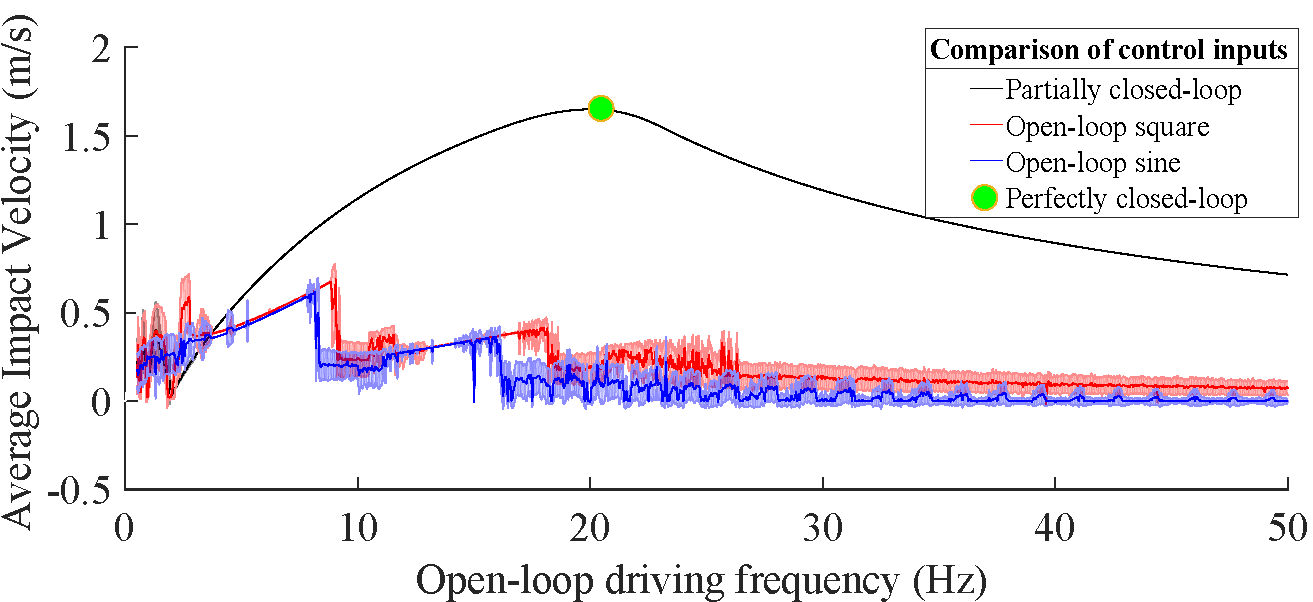
\includegraphics[width=\linewidth]{ComparisonOfControlInputs.pdf}
	\caption[Comparison of impact velocities from three control inputs]{Comparison of average impact velocities between impacts 100 and 1100 for three different control inputs: Open-loop vs. Partially closed-loop vs. Perfect closed-loop.}
	\label{CLvsOL}
	%\vspace{-1.5em}
\end{figure}
\subsection{Magnetic force calculation}
\label{magforce}

This section calculates the force applied by the magnetic field to the sphere.\par
The ferromagnetic sphere is small compared to the coil system and can be considered as a infinitely small magnetic moment $\mathbf{m}$. Assuming a constant material magnetization $\mathbf{M}$, one can calculate $\mathbf{m}$ from \cref{mag}.

$V$ is the volume of the sphere.
The ferromagnetic sphere is magnetized by the externally applied field $\mathbf{H}_{\text{app}}=\mathbf{B}_{\text{app}}/\mu_0$. Ferromagnetic materials create a demagnetizing field $\mathbf{H}_d$ when subjected to an external field. The actual field $\mathbf{H}$ seen by the sphere is the sum of $\mathbf{H}_{\text{app}}$ and $\mathbf{H}_d$. This effect must be taken into account to calculate the magnetization accurately. $\mathbf{H}_d$ is related to $\mathbf{H}_{\text{app}}$ by \cref{hd}. The demagnetization factor $N$ for a sphere is -1/3. Its magnetization can be calculated using \cref{mag2}.
Once the magnetic moment $\mathbf{m}$ is obtained, the force on the sphere can be calculated using \cref{force}.
\vspace{-2em}

\begin{align}
\mathbf{m}&=\mathbf{M}\cdot V \label{mag}\\
\mathbf{H}_d&=N\cdot \mathbf{H}_{\text{app}}\label{hd}\\
\mathbf{M}&=\frac{\mathbf{H}_{\text{app}}\left ( \mu_r-1  \right )}{2\cdot N\cdot \mu_r-1} \label{mag2}\\
\mathbf{F}&=\mathbf{\nabla}(\mathbf{m}\cdot \mathbf{B}) \label{force}
\end{align}

\subsection{Simulation results}

\subsubsection{Perfect closed-loop vs. open-loop system}
\label{clol}

A numerical model was used to simulate the system dynamics for different input gradients. Average impact velocities over impacts 100 to 1,100 were compared for a perfect closed-loop pulsed input, and open-loop inputs with sinusoidal and square profiles. As seen in figure \ref{CLvsOL}, closed-loop control produces approximately three times greater average impact velocity as compared to open-loop sinusoidal and square waves, over all frequencies. As with the analytical model in Section II-A, the simulation assumes that the robot capsule does not translate along its axis. While the absolute values of impact velocity and force will be different when the capsule is free to move, the closed-loop input can still be expected to produce higher forces than open-loop inputs. Further, for a given open-loop frequency, the variation of impact velocity over multiple contacts was found to be random for both square and sinusoidal inputs. It is not possible to reach a resonant state using a constant frequency input of any form. For a given set of input parameters, there exists only one path, or control input, that enables the system to achieve resonance. 
\begin{figure}
	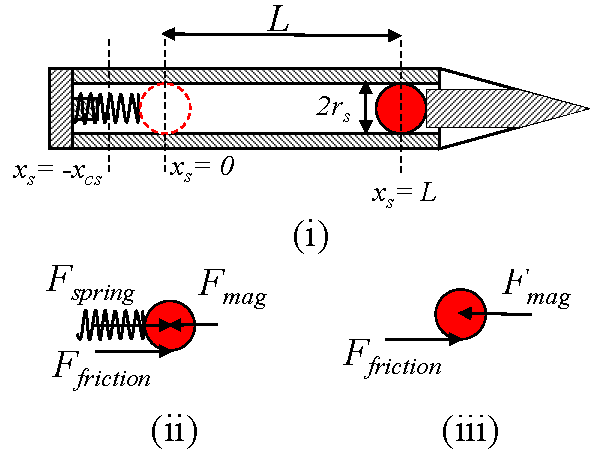
\includegraphics[width=\linewidth]{Tswitchcases.pdf}
	\caption{Six regimes for spring-end switching time; green and red represent $F_{\textrm{mag}}$ towards anterior and posterior respectively. Direction of colored arrow represents direction of ball motion.}
	\label{Tswitch}
	\vspace{-2em}
\end{figure}


\subsubsection{Partially closed-loop system}
\label{pcl}

To implement a perfect closed-loop system, sensing is required at both the spring and impact ends. While sensing at the impact end can be done using a microphone sensor (see Section \ref{partialCLexp}), it is harder to detect sphere reversal at the spring end. For experiments of the magnetic hammer on our test bench, a partially closed-loop system was implemented with only impact end sensing using a microphone. The sensor detected each impact and triggered a reversal in the direction of the gradient force. The switching time $t_s$ at the spring end was manually set at different values. The motion of the sphere between two successive impacts is analyzed based on $t_s$, the initial velocity $v_{0^+}$, and the time between impacts $\Delta t_{\textrm{imp}}$. The motion can be divided into six regimes based on $t_s$, for a given set of geometric and material properties as shown in \cref{Tswitch}. In \cref{Tswitch}(i), $v_{0^+}$ and $t_s$ are low enough that the sphere reverses direction before reaching the spring. In this case, $v_{0^+} < 2aL$, where $a=F_{\textrm{mag}}/m_s$. Fig. \ref{Tswitch}(ii) represents the case when $v_{0^+}$ is high enough that spring compression is unavoidable even for $t_s = 0$. In \cref{Tswitch}(iii), the signal switch happens after spring compression starts but before it bottoms out. Fig. \ref{Tswitch}(iv) represents perfect closed-loop switching. In \cref{Tswitch}(v), the signal is switched after maximum compression, but before the sphere reaches $x_s=0$. Fig. \ref{Tswitch}(vi) represents switching after spring rebound and before the next impact. There is also a possible seventh case where the switching happens after one entire impact cycle. This case is not relevant and serves more as an upper limit of practical $t_s$ values. 

Simulations were done for the partially closed-loop system to identify effects of different $t_s$ and $v_{0^+}$ values on $\Delta t_{\textrm{imp}}$. Fig. \ref{delTvsTs} shows $\Delta t_{\textrm{imp}}$ as a function of $t_s$ for different values of $v_{0^+}$. For $v_{0^+}=0.15\text{ m/s}$, there is a linear increase in $\Delta t_{\textrm{imp}}$ untill $t_s$ reaches a critical point. This linear region represents the case shown in \cref{Tswitch}(i). Beyond this, $\Delta t_{\textrm{imp}}$ decreases with increasing $t_s$ (\cref{Tswitch}(ii),(iii)), until the latter reaches its perfect closed-loop value. At this point $\Delta t_{\textrm{imp}}$ reaches a minimum value (\cref{Tswitch}(iv)). As $t_s$ increases beyond this, the $\Delta t_{\textrm{imp}}$ keeps increasing (\cref{Tswitch}(v),(vi)), until it saturates because the signal is switched after the duration of the entire impact cycle. The linear range does not exist for higher values of $v_{0^+}$. Future work will involve designing a control law that will help push $t_s$ values closer to perfect closed-loop values for subsequent impacts.

\begin{figure}
	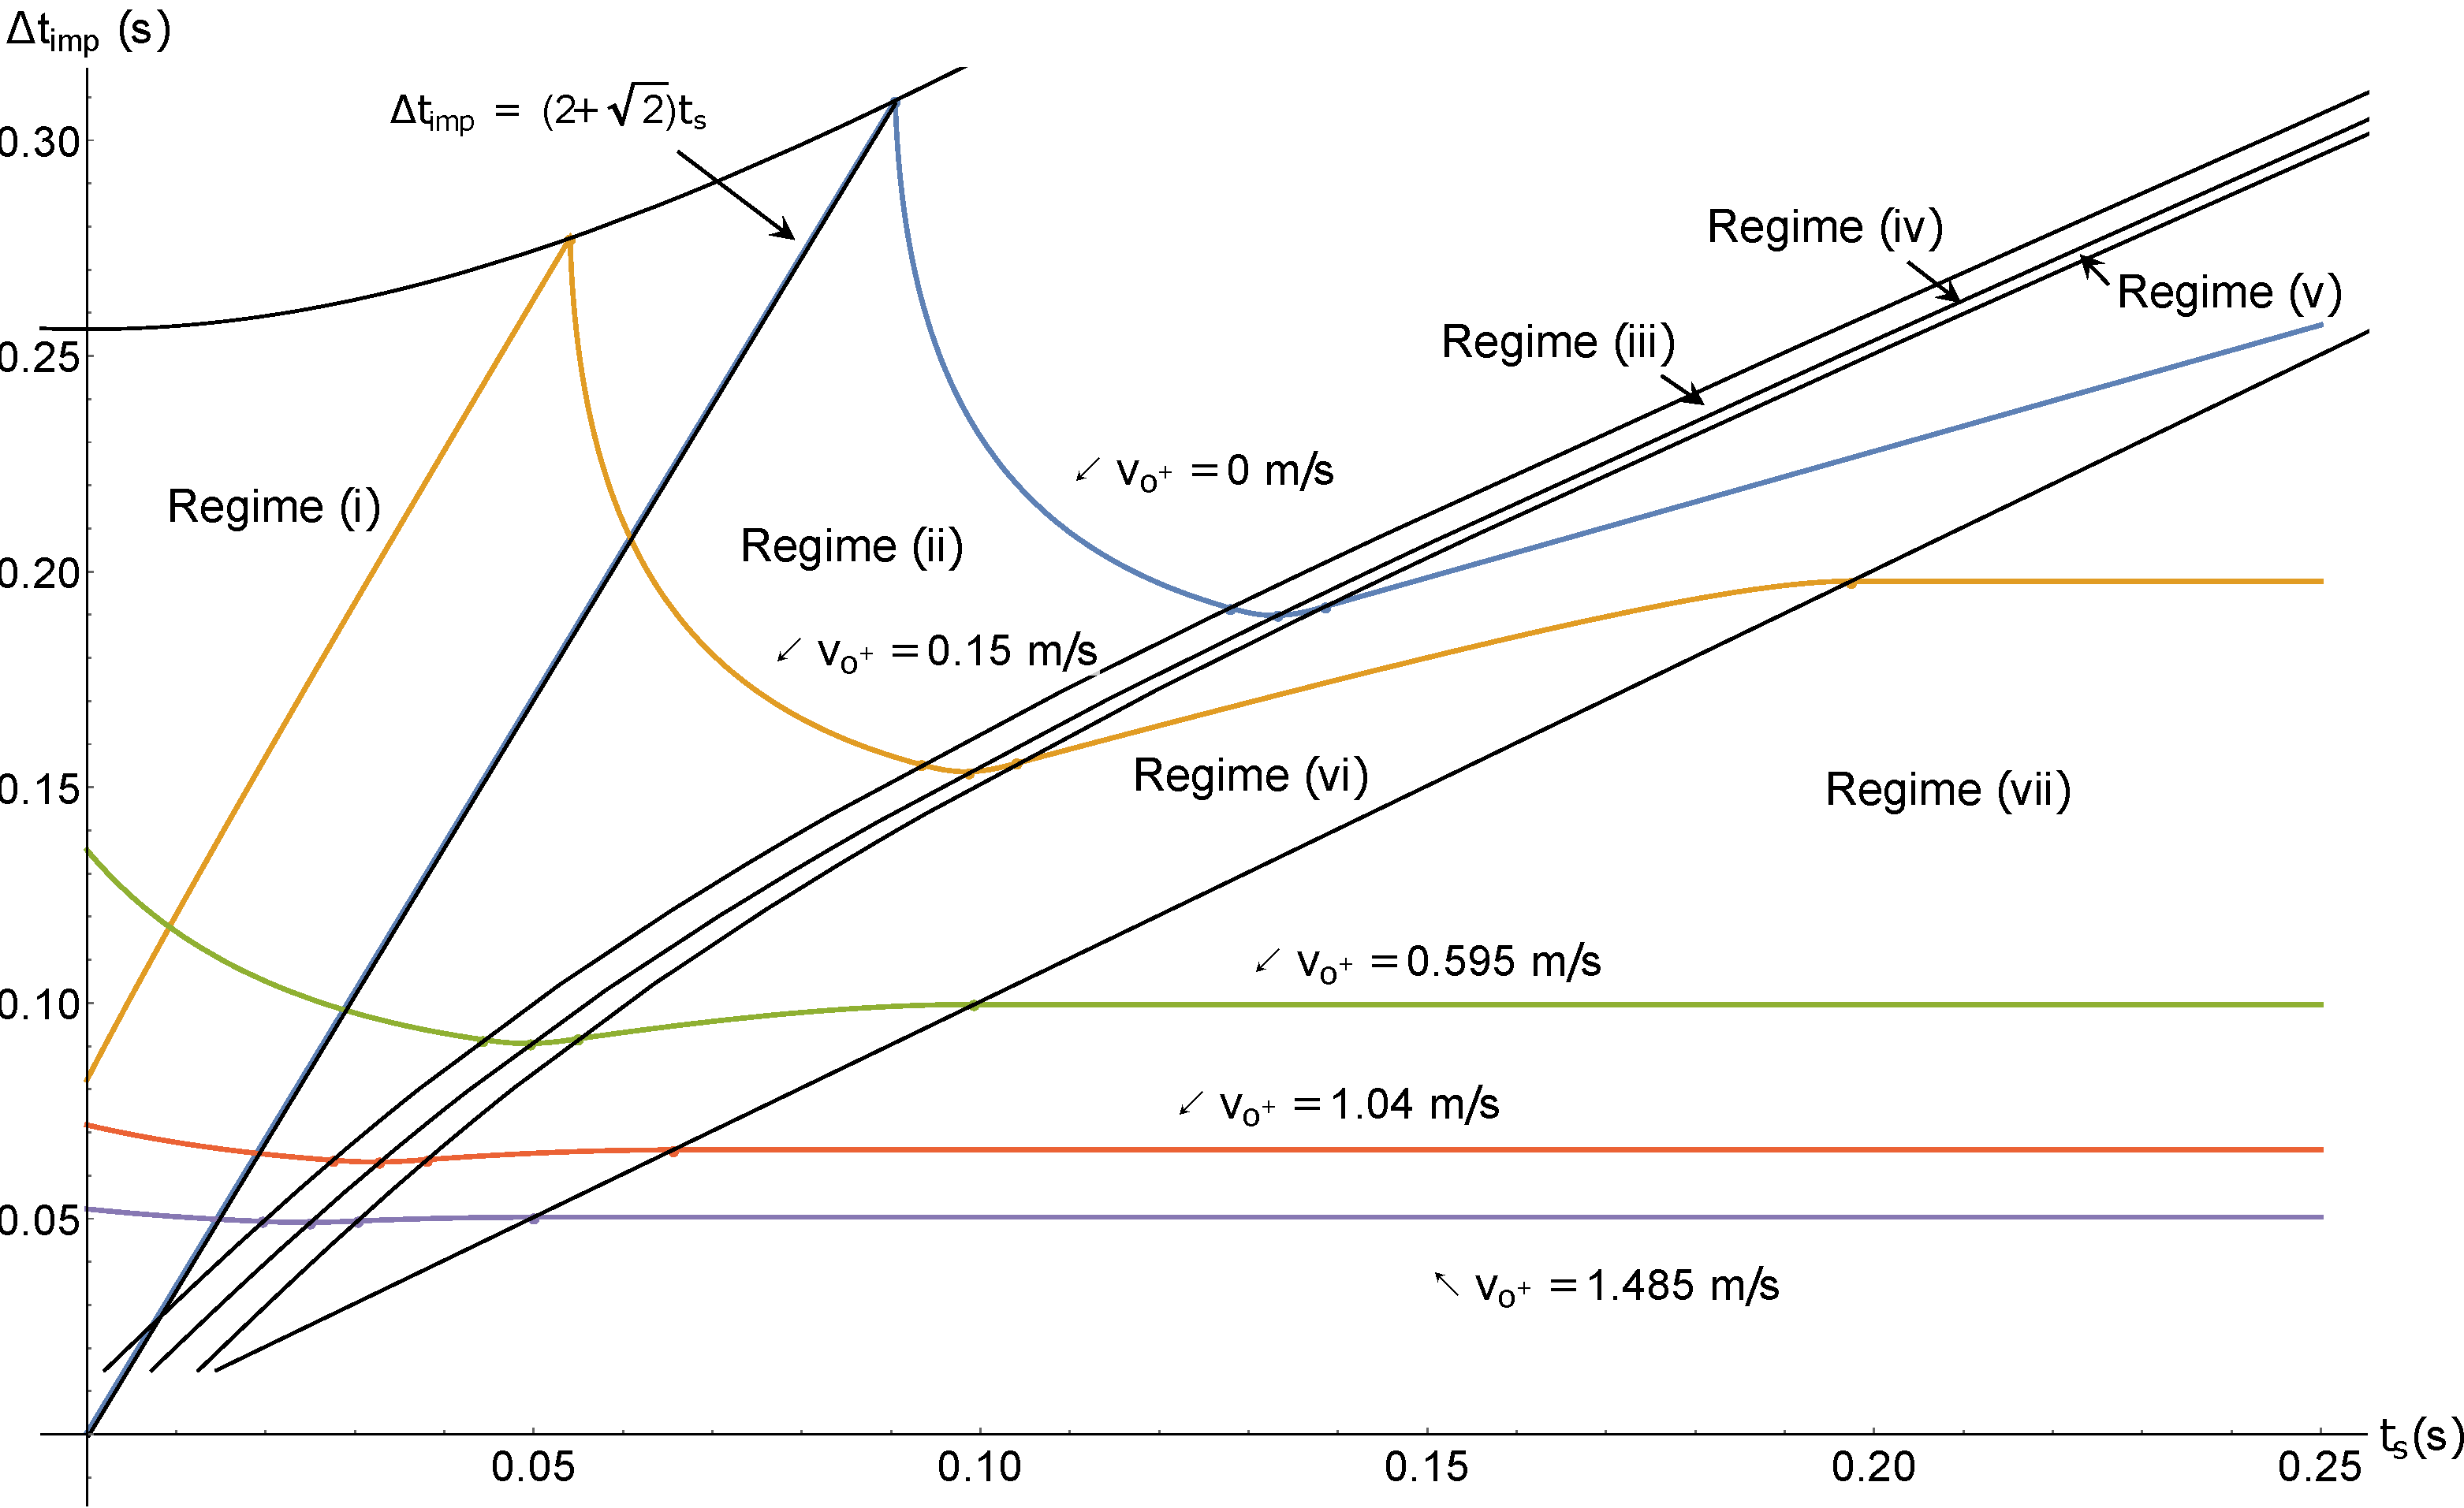
\includegraphics[width=\linewidth]{deltVsts_differentVop.pdf}
	\caption[Variation of time between impacts with switching time for partially closed-loop control]{Plot of $\Delta t_{\textrm{imp}}$ vs. $t_s$ for different values of $v_{o^+}$.}
	\label{delTvsTs}
	\vspace{-0.5em}
\end{figure}


\subsubsection{Effect of Coulomb friction}
\label{frictionwriteup}
\begin{figure}
	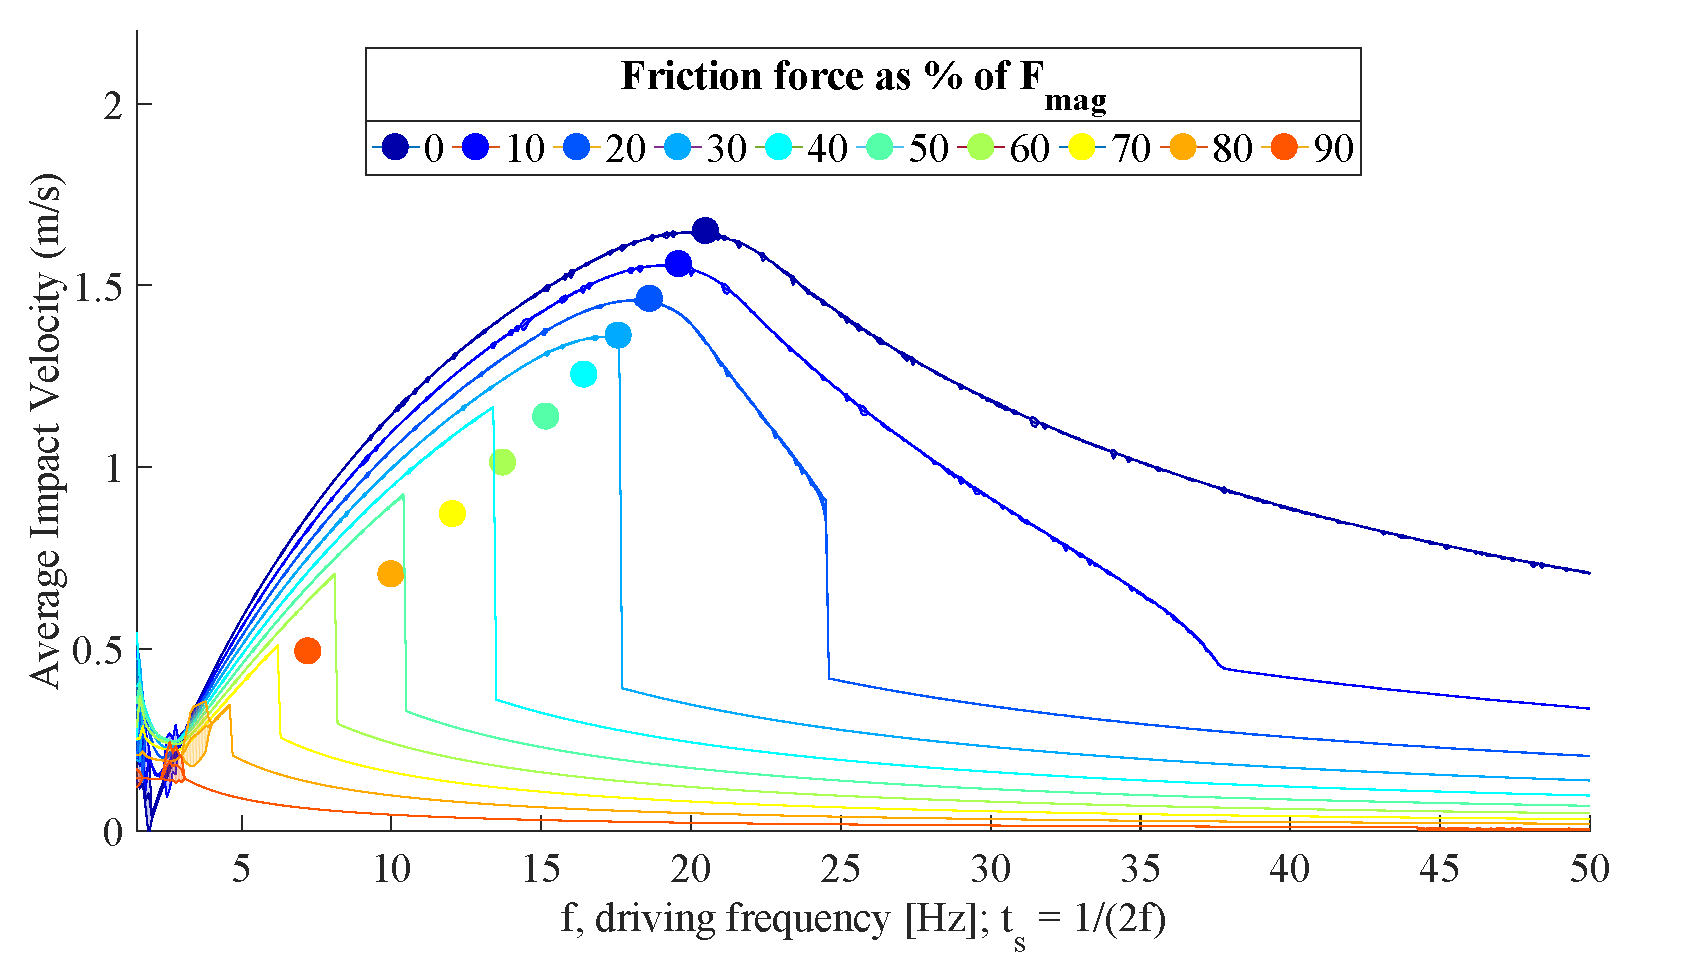
\includegraphics[width=\linewidth]{FrictionForceWithClosedLoopValues.pdf}
		\caption[Effect of Coulomb friction on partially closed-loop control]{Comparison of  simulated impact velocities. The  velocities for impacts 100 to 200 are averaged and plotted for different values of Coulomb friction force. Colored circles represent the perfect closed-loop values.  Lines represent the partially closed-loop values.}
	\label{friction}
	\vspace{-2em}
\end{figure}
In all the above models, the friction force was assumed to be zero. Average impact velocities over 100 impacts are plotted for varying values of the friction force in Fig. \ref{friction}. The circles represent the perfect closed-loop values, while the curves represent the partially closed-loop values using impact times. Much like the step-out frequency of a stepper motor, average impact velocities drop suddenly for the partially closed-loop system beyond a cut-off driving frequency. This is due to the sphere reversing direction before spring contact, leading to a drop in its net kinetic energy. As friction force increases as a percentage of $F_{\textrm{mag}}$, the partially closed-loop system reaches its cutoff frequency, before resonance. This drop in impact velocity is not seen in the perfect closed-loop system for any values of friction since the spring is always compressed to its maximum limit. Hence, partially closed-loop control will not produce the maximum possible impact velocity for high values of Coulomb friction force. Future work will use better models of kinetic and static friction, as well as air resistance.

\section{Experimental determination of Impact coefficient of restitution}
\label{cor_det}
The coefficient of restitution $e$ was determined using the time interval between two consecutive bounces of the sphere when dropped from a given height onto the impact rod. The measurements were made using 38.1 mm long impact rods for five different materials. Impact rods were held by a drill chuck. A length of 10.0 mm of the impact rods was sticking out of the chuck. The experimental setup is shown in \cref{CoR_setup_data}.

The results, shown in fig. \ref{CoR_setup_data} (c), show that titanium offers the largest coefficient of restitution. The densities of aluminum, titanium, stainless steel, brass, and copper are 2720, 4500, 7600, 8500, and 8940 kg/m$^3$ respectively. This data, coupled with a desire for a lightweight millirobot suggests that titanium is the best material for an impact plate. Bio-compatibility of the material used is another constraint.

\begin{figure}
	\includegraphics[width=\columnwidth]{CoR_setup_data.pdf}
	\caption{(a) Microphone output showing multiple bounces of sphere (b) Experimental setup for measuring the coefficient of restitution, $e$ (c) Measured values of $e$ for different materials and rod diameters. 10 measurements were performed for each data points.}
	\label{CoR_setup_data}
	\vspace{-1.5em}
\end{figure}




\section{Experimental magnetic hammer tests}
\label{experiment}
\subsection{Magnetic test bench description}

A desktop-size, single-axis magnetic setup was built to reduce the cost related to clinical MRI experiments.
 It is composed of two solenoid coils oriented along the same axis and separated by a distance $d$. 
 The coils are used to produce both the magnetizing field and the gradient. 
 The properties of the coils are shown in Table \ref{coil_table}.\par
The system is shown in \cref{magnetic_setup}.
 The two coils are held by an acrylic tube. 
 They can slide along this tube and be locked in place to adjust the distance between the two coils and therefore change the maximum field and gradient values. 
 The acrylic tube is transparent, allowing for visual access to the robot.
Each coil is powered by a Syren 25 regenerative switching power supply. The Syren 25 are manufactured by Dimension Engineering. They can provide continuously a current of 25 A with a maximum voltage of 24 V.\par
Robots are inserted inside the acrylic tube holding the coils. 
They are held by a second, smaller tube that guides them along the system axis. 
Robots can be free to move along the coil axis or held in place. 
A picture of the system is provided in \cref{magnetic_setup}.

\begin{figure}
	\begin{centering}
  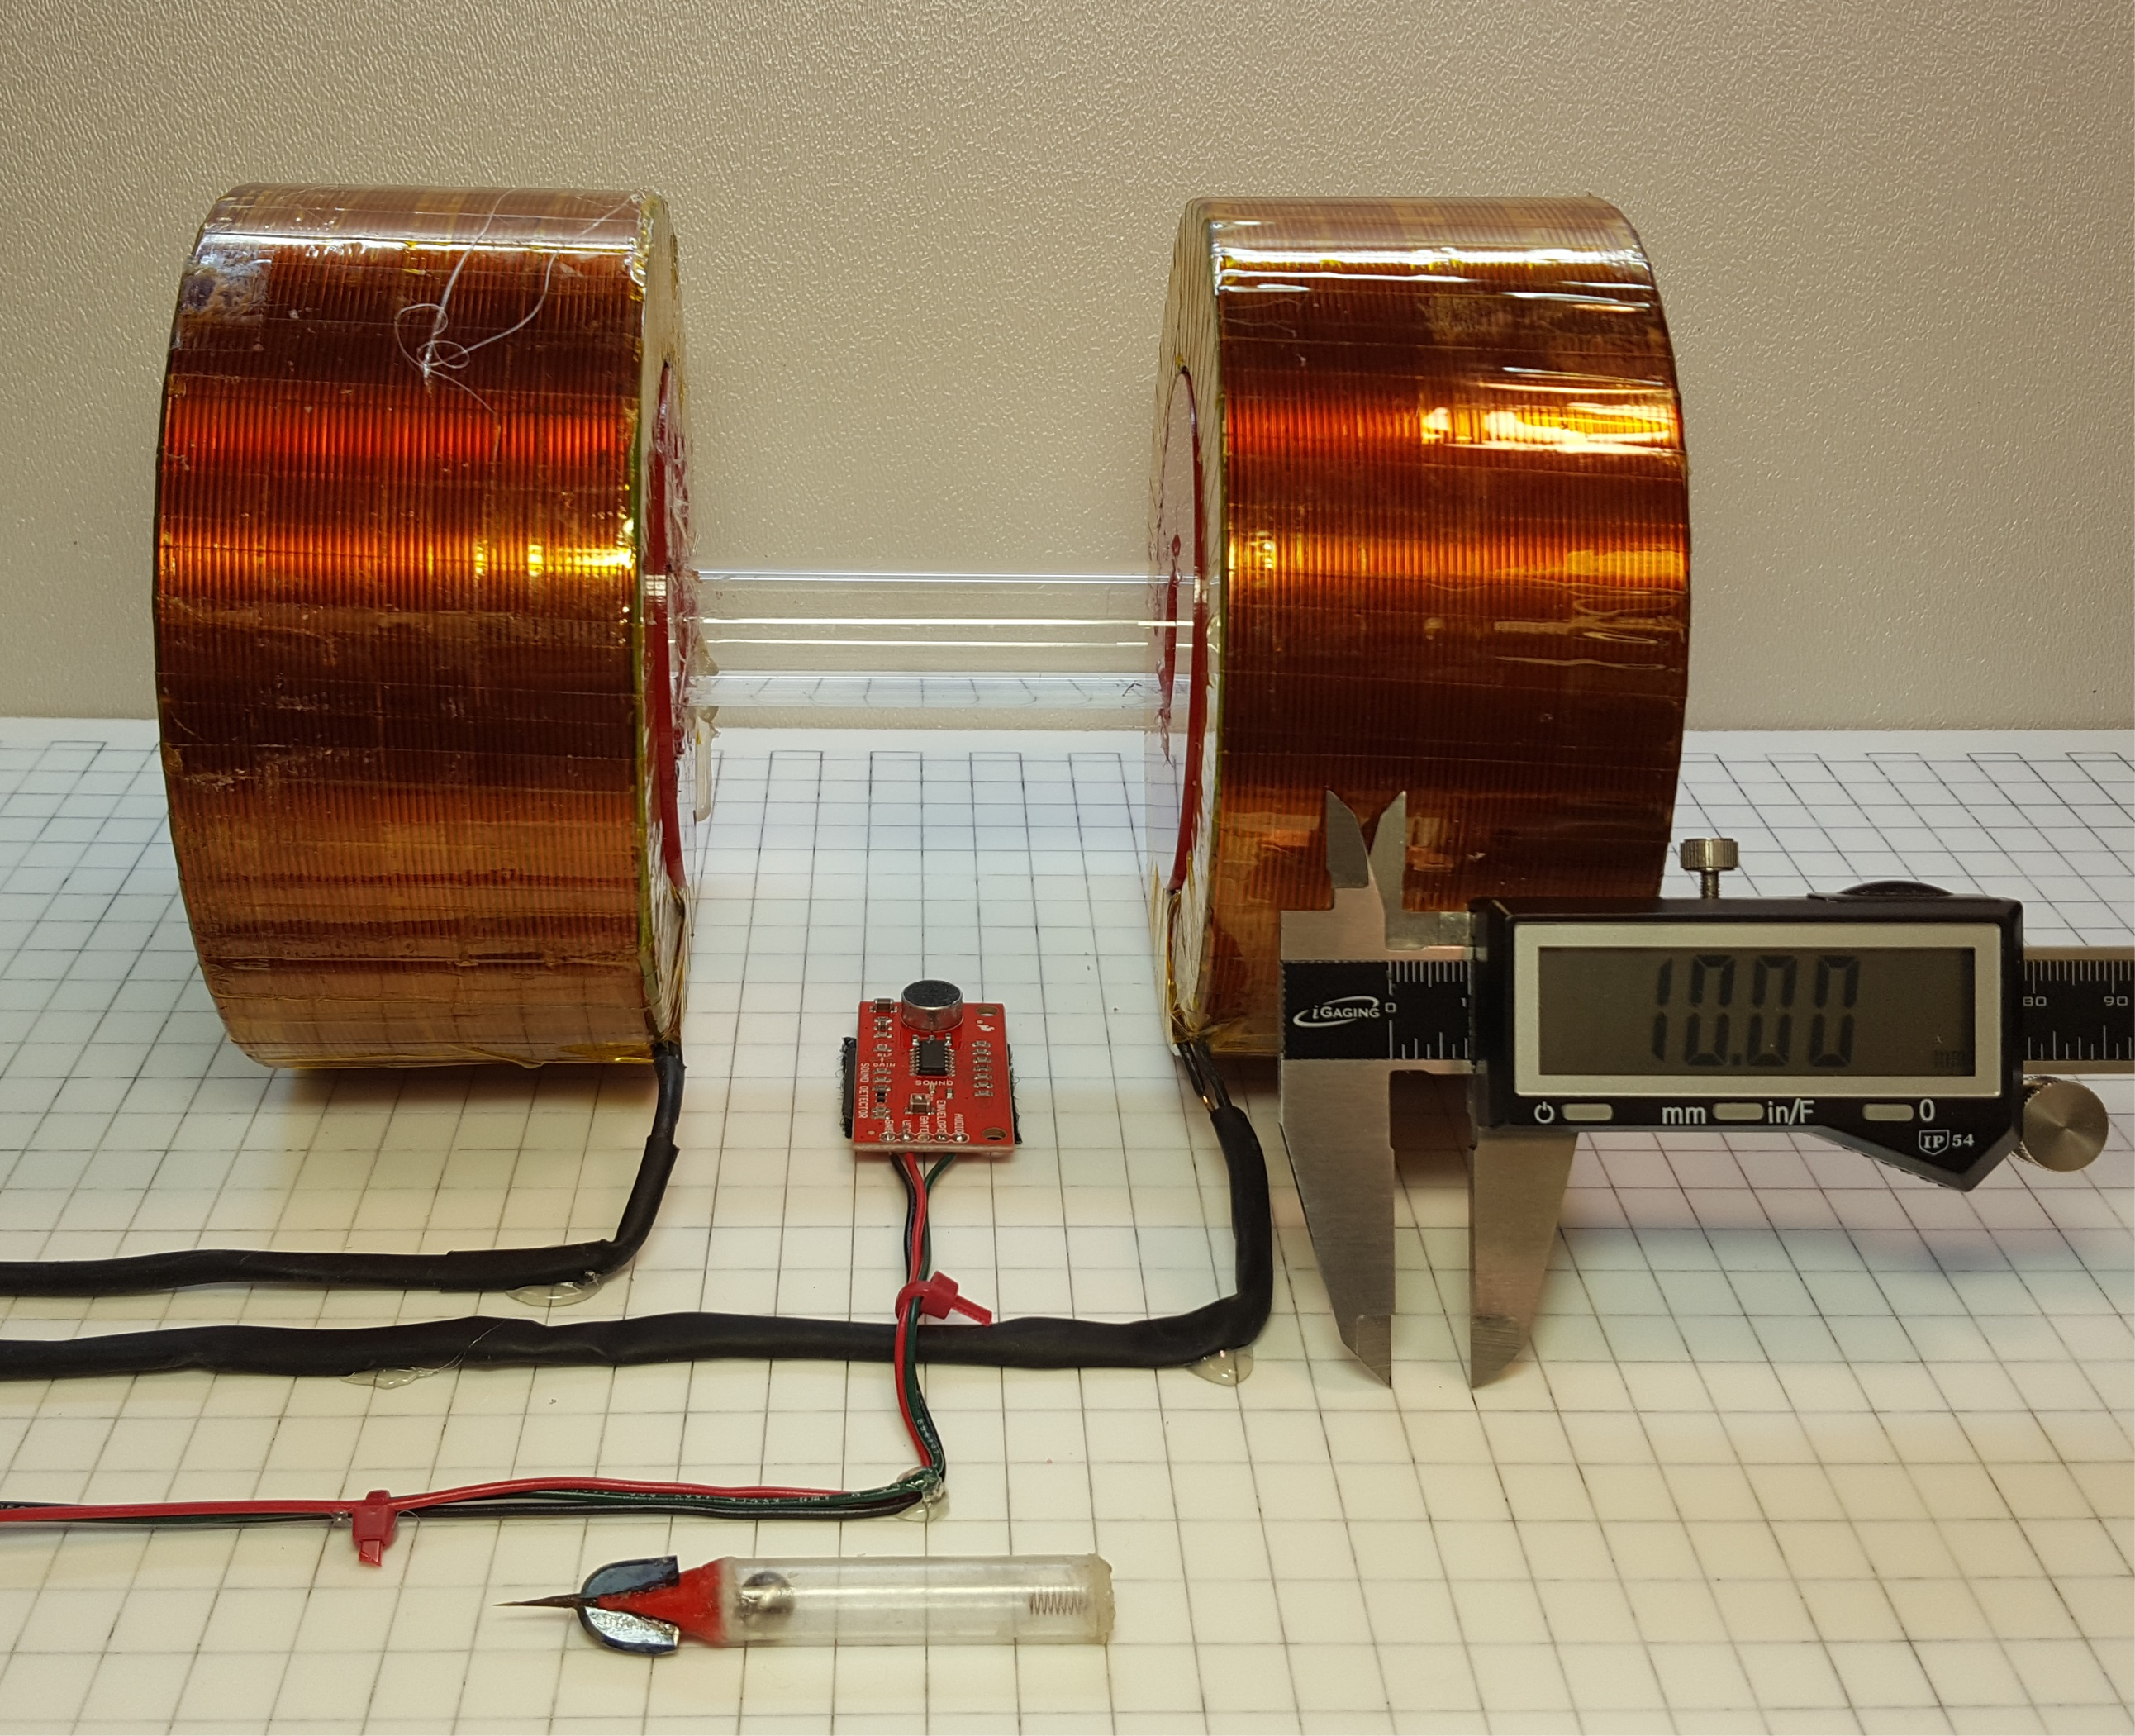
\includegraphics[width=165pt]{Magnetic_test_bench.jpg}
  \caption{Picture of the magnetic test bench.}
  \label{magnetic_setup}
	\end{centering}
	\vspace{-0.5em}
\end{figure}


\begin{table}[]
\centering
\caption{Properties of the coils used in the magnetic test bench}
\label{coil_table}
\scalebox{0.95}{%
\begin{tabular}{|l|l||l|l|}
\hline
Internal Radius    & 140 mm                   & Electrical resistance                                                                      & 8.17 $\Omega$       \\ \hline
External Radius    & 63 mm                   & Inductance                                                                                 & 113 mH    \\ \hline
Length             & 60 mm                     & \begin{tabular}[c]{@{}l@{}}Max current change rate \\ Voltage = 25 V\end{tabular}          & 130 A/s \\ \hline
Wire               & 18 AWG                    & Max continuous current                                                                 & 10 A       \\ \hline
Wire cross-section & 0.823 mm$^2$ & \begin{tabular}[c]{@{}l@{}}Flux density on \\ system center\\ I = 10 A, $d$ = 50 mm\end{tabular} & 55 mT      \\ \hline
Number of turns    & 265                       & \begin{tabular}[c]{@{}l@{}}Gradient on \\system center\\  I = 10 A, $d$ = 50 mm\end{tabular}    & 0.14 T/m   \\ \hline
\end{tabular}}
\vspace{-1.5em}
\end{table}


\subsection{Partially closed-loop experiment}
\label{partialCLexp}
A system to record the impact velocity of the sphere as well as the driving period of the magnetic hammer was built. A schematic representation of the system is shown in fig. \ref{laser_system}. The main body of the system is a 3d printed tube with thick walls. The sphere is a NdFeB permanent magnet with a magnetization of 883,000 A/m. It has a mass of 1.05 g. It is placed inside the tube and an impact rod and a spring are placed on the anterior and posterior sides respectively. This constitutes the magnetic hammer system. A laser and a diametrically opposed light sensor are placed radially on the tube, with radial holes in the tube for the laser beam to pass through. The thick walls of the tube permit the encapsulation of the laser and the sensor with epoxy resin.\par

\begin{figure}
    \centering
  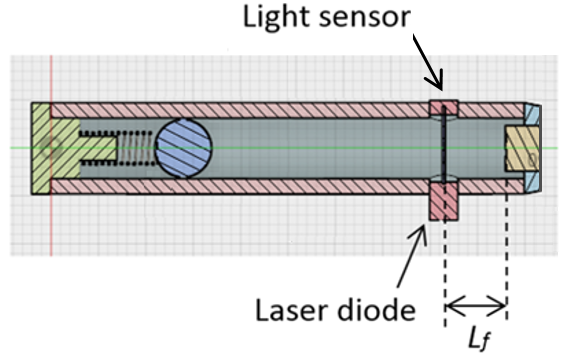
\includegraphics[width=120pt]{laser_system.png}
  \caption{Schematic representation of the system using a laser and a light sensor to measure the sphere velocity}
  \label{laser_system}
	%\vspace{-2em}
\end{figure}

When moving, the sphere interrupts the laser beam during a time $t_i$ inversely proportional to the velocity. By measuring $t_i$ one can calculate the average velocity $V$ of the sphere with $V=2\cdot r_s/t_i$. The laser beam was positioned on the anterior side of the capsule, mounted at a distance $L_f>2r_s$ from the impact rod to allow the sphere to not interrupt the beam when it touches the impact rod. This positioning enables computing the velocity of the sphere just before the impact which we will consider as being equal to the impact velocity. The acquisition of the data is automatic and performed via a National Instrument cRIO real-time controller. The controller was programmed using LabVIEW.\par 
The cRIO is used at the same time to control the magnetic hammer. The partially closed-loop method is used. Square shaped current waveform drive the coils. The current in the coils either either considered to be $I_{\textrm{max}}$ or 0 A. The time constant of the coils (13 ms) is small enough compared to $T_s$ to neglect the current transient. The coil will be said to be ``on'' when $I=I_{\textrm{max}}$ and ``off'' when $I=0$ A. A microphone is used to monitor the noise produced by the system. The impact creates a large pulsed signal on the microphone output that can be easily detected. When the impact is detected, the anterior coil is turned off while the posterior coil is turned on. The force applied to the sphere pushes it toward the posterior side. The current stays constant during a time $t_s$ after the impact is detected. The anterior coil is subsequently turned on, and the posterior coil is turned off. The force then pushes the sphere forward. The current in the coils is changed again when another impact is detected. This process is repeated indefinitely.\par

\begin{figure}
  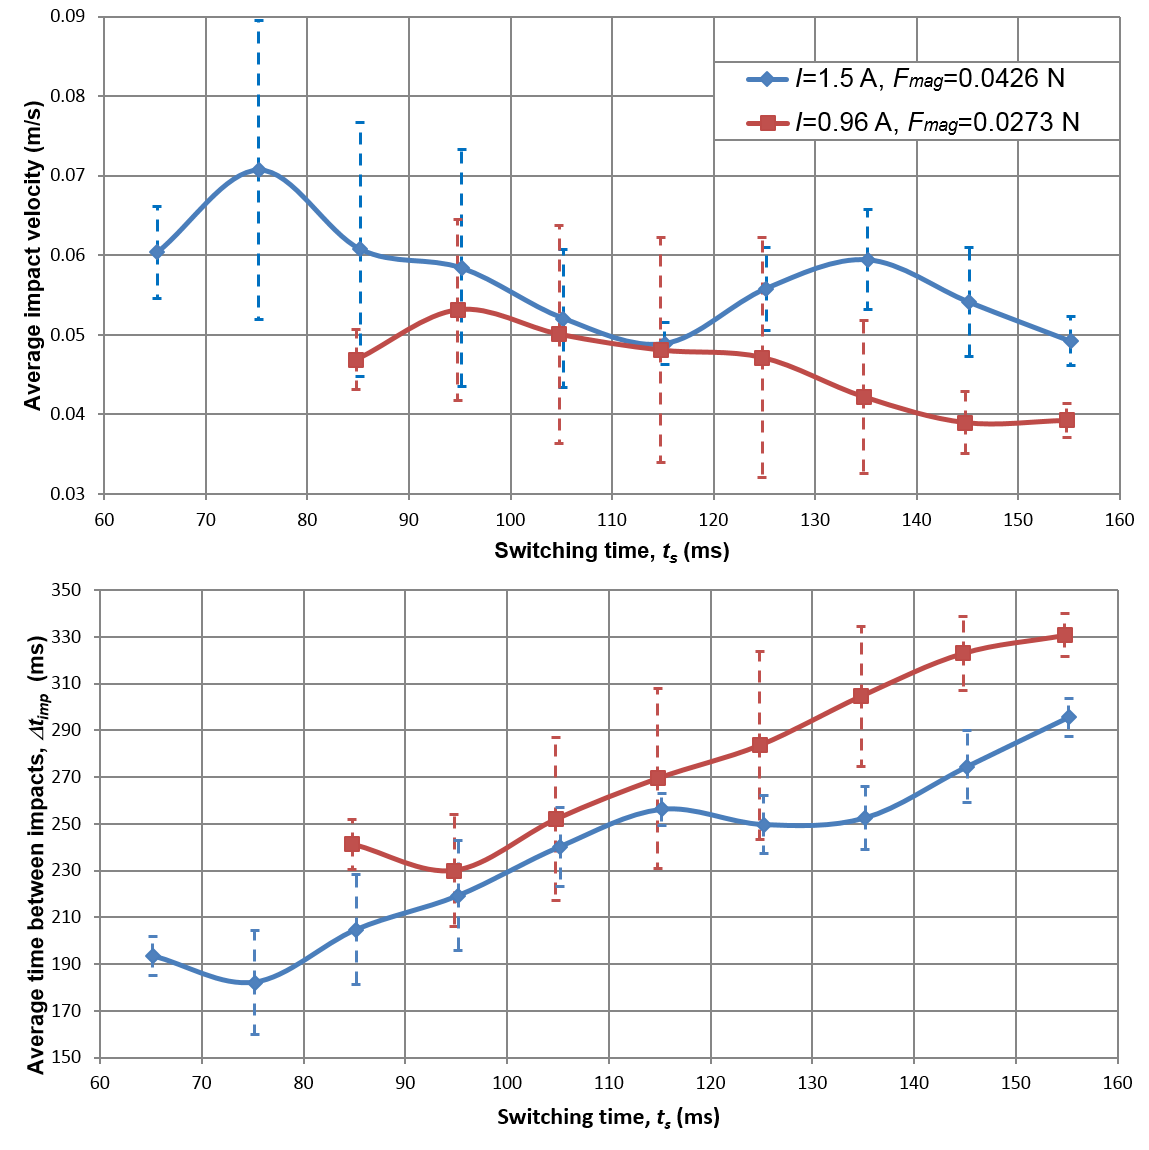
\includegraphics[width=\linewidth]{laser_exp.png}
  \caption{Experimental results obtained with the laser-based sensor. The error bars represent the standard deviation. 300 impacts were recorded for each point.}
  \label{laser_exp}
	\vspace{-2em}
\end{figure}

Data were recorded for $I_{\textrm{max}}$ values of 0.96A, 1.5A and 2.2A which correspond to forces $F_{\textrm{mag}}$ equal to 0.0273N, 0.0426N and 0.0625N respectively. The value for $F_{\textrm{mag}}$ were calculated using the software FEMM. Results of the measurements are presented in fig. \ref{laser_exp}. The impact velocity is larger at 1.5A than at 0.96A due to the larger force exerted on the sphere at larger current. This increase in velocity produces a decrease on the average time between impact $\Delta t_{\textrm{imp}}$ (on the bottom curve, one can see that $\Delta t_{\textrm{imp}}$ is smaller for the largest current). These curves exhibit a maximum impact velocity, at $t_s=75$ ms for $I_{\textrm{max}}$=1.5 A and $t_s=95$ ms for $I_{\textrm{max}}$=0.96A. These points coincide with a minimum on the $\Delta t_{\textrm{imp}}$ curve and correspond to the optimal driving frequency. The curve measured at higher current, 2.2A, show better performance overall in both impacts per second and velocity. A few points are not in agreement with this observation but the difference is within the value of the standard deviation. At all current values, our visual observations as well as the large standard deviation indicates that the control with the partially closed-loop method is not optimum because it is not able to maintain the maximum velocity for each impact.\\
The impact velocity has a local maximum at $t_s$=135 ms for the curve at measured at 1.5A. This is a point where the system exhibits another resonance, when the sphere compresses the spring two times during each cycle.

\section{Preliminary tests in clinical mri}
\label{MRI_tests}
Preliminary tests of magnetic hammers were performed in a clinical 3T Siemens MRI scanner to demonstrate the ability of MRI scanners to produce a force able to drive the device.
No closed-loop control was implemented. 
The magnetic gradient  oscillated at a constant frequency. 
As seen before, the system does not work optimally in these conditions. 
At low frequencies, the magnetic sphere completely stops on both sides of the millirobot. 
All the kinetic energy is lost at these times, and the magnetic hammer, therefore, performs poorly. 
The aim of these tests is to prove that MRI scanners are suitable to produce the desired force on the magnetic sphere inside the millirobot and provide a pulsed force.\par
A 50 mm long, 7 mm diameter robot was built for this test. The sphere has a diameter of 5mm and is made of stainless steel. This material is used instead of a permanent magnet because the main magnetic field of the MRI scanner magnetizes the stainless steel at its saturation value which is higher than the magnetization of a permanent magnet.\par
A plastic container was placed inside the MRI scanner, sitting on the patient table. The millirobot was positioned inside this container, with its length oriented along the $x$ axis. The tissue sample to penetrate was a goat brain hemisphere placed in the container, in front of the millirobot tip. .
A 2 Hz square gradient along the $x$ axis with an amplitude of 23 mT/m was applied to it. 
This frequency is slow enough to allow the sphere to stop on both sides completely. \par
Friction with the plastic container prevented the capsule from moving when a constant gradient was applied. Once the gradient wave was started, the sphere began to move back and forth while the robot was moving toward the sample at each impact, at an average speed of 1.9 mm/s. 
 The robot then began to penetrate the sample. It went 9 mm deep inside it and stopped progressing (see \cref{MRI_test}). 
This experiment demonstrates the suitability of MRI scanners to drive magnetic hammers. No further measurements were made as this demonstration was the sole purpose of the experiment and the magnetic test bench allows us to perform extensive testing at reduced cost.\par
Future work will implement closed-loop control on the clinical MRI scanner to transfer energy efficiently. 
The MRI signal could be used to compute the position of the magnetic sphere at a frequency greater than 20 Hz, as we did in~\cite{578}.

\begin{figure}
\centering
  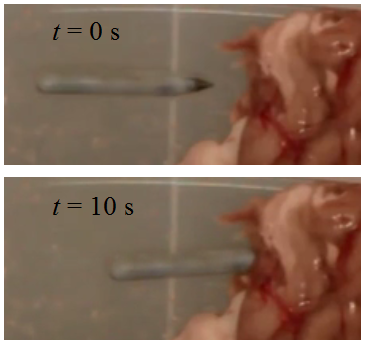
\includegraphics[width=120 pt]{tests_in_MRI.png}
  \caption{Picture of the magnetic hammer driven by an MRI scanner. The penetration test is realized on a goat brain sample.}
  \label{MRI_test}
	\vspace{-2em}
\end{figure}

\section{Tissue penetration experiment}

An iterative design process was used to achieve tissue penetration using the magnetic test bench. Seven millirobots were built and tested, varying the tip shape and composition, the tube length, the spring, and the sphere material. \par
Our observations of the penetration experiments concluded that sharp blades placed on the tip of the millirobot allow for an easier tissue penetration. The blades are placed much like on a hunting arrow tip, and create a fissure in the tissue that reduces the force needed for the capsule to progress through the sample. The blades used in our experiments were made of titanium, a bio-compatible and non-magnetic metal.\par
Our observations also showed that, when the sphere compresses the spring, the capsule tends to move backward. This effect releases the pressure exerted by the millirobot tip on the tissue and therefore makes the impact less efficient at penetrating the sample. This issue was solved by placing a porcupine needle placed at the leading tip of the millirobot, at the center of the blades. Porcupine needles are covered with microscopic backward facing barbs. These barbs prevent the needle from being pulled off a tissue once penetrated. Natural porcupine needles cannot be sanitized and so cannot be used in an in-vivo medical intervention. However, synthetic porcupine needles can be built \cite{cho2012microstructured}.\par

\begin{figure}
	\centering
  \includegraphics[width=150pt]{brain_penetration.png}
  \caption{Picture presenting the penetration of a millirobot prototype inside a lamb brain sample. The corresponding video is attached to this paper.}
  \label{brain_penetration}
	\vspace{-1.5em}
\end{figure}

Fig. \ref{brain_penetration} show frames of a video from a representative penetration test. A video attached to this paper shows this test. The tissue samples used in these experiments were 10 mm thick lamb brain slices. As shown in the attached video, it was placed in a sample holder made with two acrylic sheets, one on each side. Two holes in the sample holder allow the millirobot to access and cross the tissue. The millirobot used in this experiment has a diameter of 7.5 mm. It uses three titanium blades, a porcupine needle, and a titanium impact rod. The sphere is a NdFeB permanent magnet with a 6.35 mm diameter and a mass of 1.05 g. The spring has a free length of 10 mm and a constant of 35 N/m. The free length of sphere travel is 15 mm. The flux density applied by the coils had a maximum value of 40 mT and a maximum gradient of 545 mT/m. The control was performed with the partially closed-loop method presented in Section \ref{pcl}.\par
We performed a series of four successful penetration tests with no failures using our final millirobot design. The first three samples were perforated in 225, 252 and 230 seconds. It took 20 minutes for the millrobot to perforate the fourth sample because it included the \emph{pia mater}. These tests prove the capability of the magnetic hammer system to penetrate biological tissue.
\vspace{-1em}
\section{CONCLUSIONS}
\label{conclusion}
A magnetic hammer system for a millirobot driven by the gradient fields of an MRI scanner was studied. 
The system enables producing force large enough to penetrate body tissue.
The hammer is composed of a magnetic sphere moving inside a tube.\par
A modelization allows the computation of the position of the sphere as a function of time. 
The magnetic flux density and the gradient are computed using a semi-analytical method and allow an accurate calculation of the force applied to the sphere. A study about the sphere friction on the tube was performed. The friction between the air and the sphere was not taken into account as the final millirobot will be under vacuum to prevent any air release within the body.
The speed of the sphere after impact is computed from the coefficient of restitution. \par
The coefficient of restitution ($e$) depends on the materials of the colliding objects and also on their shape and sizes. 
Values of $e$ were experimentally measured. 
These measurements showed that titanium impact plates exhibit large values of $e$. 
This material also has the advantage of being lightweight, a useful property to achieve neutral buoyancy of millirobots, and is a bio-compatible material.\par
A magnetic test bench was built to reduce experimental cost related to the use of a clinical MRI scanner. 
A magnetic hammer was tested with a partially closed-loop control. 
The impact of the sphere is detected via a microphone. 
The posterior coil is turned on during a predetermined time $t_s$ to pull the sphere backward.
 After this time, the posterior coil is turned off and the anterior coil is turned on until the next impact is detected.\par
A laser based sensor was used to record the impact velocity of the sphere. The data obtained shows that there is an optimum value for $t_s$ where the impact velocity is maximum. The impact velocity also increases when the magnetic field value increases.\par
	In a series of four trials the magnetic test bench propelled a millirobot through lamb brain samples. Preliminary tests in a 3T MRI scanner validated the mechanical design. Future work should implement and test closed-loop control of the magnetic hammer in a clinical MRI scanner, detecting impacts with the MRI signal instead of a microphone. 
Tradeoffs involved in miniaturization of the robot should also be studied.
\vspace{-1.1em}
 

\addtolength{\textheight}{-12cm}   % This command serves to balance the column lengths
                                  % on the last page of the document manually. It shortens
                                  % the textheight of the last page by a suitable amount.
                                  % This command does not take effect until the next page
                                  % so it should come on the page before the last. Make
                                  % sure that you do not shorten the textheight too much.

%%%%%%%%%%%%%%%%%%%%%%%%%%%%%%%%%%%%%%%%%%%%%%%%%%%%%%%%%%%%%%%%%%%%%%%%%%%%%%%%



%%%%%%%%%%%%%%%%%%%%%%%%%%%%%%%%%%%%%%%%%%%%%%%%%%%%%%%%%%%%%%%%%%%%%%%%%%%%%%%%

\bibliographystyle{unsrt}
\bibliography{biblio}



\end{document}
